\documentclass[10pt]{article}
\usepackage[polish]{babel}
\usepackage[utf8]{inputenc}
\usepackage[T1]{fontenc}
\usepackage{graphicx}
\usepackage[export]{adjustbox}
\graphicspath{ {./images/} }
\usepackage{amsmath}
\usepackage{amsfonts}
\usepackage{amssymb}
\usepackage[version=4]{mhchem}
\usepackage{stmaryrd}
\usepackage{multirow}

\title{EGZAMIN MATURALNY }

\author{}
\date{}


\begin{document}
\maketitle
\begin{center}
\begin{tabular}{|c|}
\hline
Miejsce \\
na naklejkę \\
z kodem szkoly \\
\hline
\end{tabular}
\end{center}

\begin{center}

\includegraphics[max width=\textwidth]{2024_11_21_9c6d19831f6022e8f7beg-01(1)}
\end{center}

Z MATEMATYKI

\section*{POZIOM ROZSZERZONY}
MAJ\\
ROK 2007

\section*{Czas pracy 180 minut}
\section*{Instrukcja dla zdającego}
\begin{enumerate}
  \item Sprawdź, czy arkusz egzaminacyjny zawiera 15 stron (zadania \(1-11\) ). Ewentualny brak zgłoś przewodniczacemu zespołu nadzorującego egzamin.
  \item Rozwiązania zadań i odpowiedzi zamieść w miejscu na to przeznaczonym.
  \item W rozwiązaniach zadań przedstaw tok rozumowania prowadzacy do ostatecznego wyniku.
  \item Pisz czytelnie. Używaj długopisu/pióra tylko z czarnym tuszem/atramentem.
  \item Nie używaj korektora, a błędne zapisy przekreśl.
  \item Pamiętaj, że zapisy w brudnopisie nie podlegają ocenie.
  \item Obok każdego zadania podana jest maksymalna liczba punktów, którą możesz uzyskać za jego poprawne rozwiązanie.
  \item Możesz korzystać z zestawu wzorów matematycznych, cyrkla i linijki oraz kalkulatora.
  \item Wypełnij tę część karty odpowiedzi, którą koduje zdający. Nie wpisuj żadnych znaków w części przeznaczonej dla egzaminatora.
  \item Na karcie odpowiedzi wpisz swoją datę urodzenia i PESEL. Zamaluj - pola odpowiadajace cyfrom numeru PESEL. Błędne zaznaczenie otocz kółkiem ( i zaznacz właściwe.\\

\includegraphics[max width=\textwidth, center]{2024_11_21_9c6d19831f6022e8f7beg-01(3)}
\end{enumerate}

Za rozwiązanie wszystkich zadań można otrzymać\\
łacznie\\
50 punktów\\
Życzymy powodzenia!

Wypelnia zdający przed rozpoczęciem pracy\\
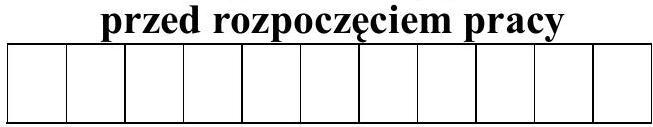
\includegraphics[max width=\textwidth, center]{2024_11_21_9c6d19831f6022e8f7beg-01(2)}

PESEL ZDAJĄCEGO\\
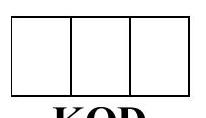
\includegraphics[max width=\textwidth, center]{2024_11_21_9c6d19831f6022e8f7beg-01}

KOD\\
ZDAJĄCEGO

\section*{Zadanie 1. (5 pkt)}
Dana jest funkcja \(f(x)=|x-1|-|x+2|\) dla \(x \in R\).\\
a) Wyznacz zbiór wartości funkcji \(f\) dla \(x \in(-\infty,-2)\).\\
b) Naszkicuj wykres tej funkcji.\\
c) Podaj jej miejsca zerowe.\\
d) Wyznacz wszystkie wartości parametru \(m\), dla których równanie \(f(x)=m\) nie ma rozwiązania.\\

\includegraphics[max width=\textwidth, center]{2024_11_21_9c6d19831f6022e8f7beg-02}

\begin{center}
\begin{tabular}{|c|l|c|c|c|c|c|}
\hline
\multirow{2}{*}{\begin{tabular}{c}
Wypełnia \\
egzaminator! \\
\end{tabular}} & Nr czynności & 1.1. & 1.2. & 1.3. & 1.4. & 1.5. \\
\cline { 2 - 7 }
 & Maks. liczba pkt & 1 & 1 & 1 & 1 & 1 \\
\cline { 2 - 7 }
 & Uzyskana liczba pkt &  &  &  &  &  \\
\hline
\end{tabular}
\end{center}

\section*{Zadanie 2. (5 pkt)}
Rozwiąż nierówność: \(\log _{\frac{1}{3}}\left(x^{2}-1\right)+\log _{\frac{1}{3}}(5-x)>\log _{\frac{1}{3}}(3(x+1))\).\\

\includegraphics[max width=\textwidth, center]{2024_11_21_9c6d19831f6022e8f7beg-03}

\begin{center}
\begin{tabular}{|c|l|c|c|c|c|c|}
\hline
\multirow{2}{*}{\begin{tabular}{c}
Wypełnia \\
egzaminator! \\
\end{tabular}} & Nr czynności & 2.1. & 2.2. & 2.3. & 2.4. & 2.5. \\
\cline { 2 - 7 }
 & Maks. liczba pkt & 1 & 1 & 1 & 1 & 1 \\
\cline { 2 - 7 }
 & Uzyskana liczba pkt &  &  &  &  &  \\
\hline
\end{tabular}
\end{center}

\section*{Zadanie 3. (5 pkt)}
Kapsuła lądownika ma kształt stożka zakończonego w podstawie półkulą o tym samym promieniu co promień podstawy stożka. Wysokość stożka jest o 1 m większa niż promień półkuli. Objętość stożka stanowi \(\frac{2}{3}\) objętości całej kapsuły. Oblicz objętość kapsuły lądownika.\\

\includegraphics[max width=\textwidth, center]{2024_11_21_9c6d19831f6022e8f7beg-04}

\section*{Zadanie 4. (3 pkt)}
Dany jest trójkąt o bokach długości \(1, \frac{3}{2}, 2\). Oblicz cosinus i sinus kąta leżącego naprzeciw najkrótszego boku tego trójkąta.

\begin{center}
\begin{tabular}{|c|c|c|c|c|c|c|c|c|c|c|c|c|c|c|c|c|c|c|c|c|c|c|c|c|c|c|c|c|c|c|c|}
\hline
 &  &  &  &  &  &  &  &  &  &  &  &  &  &  &  &  &  &  &  &  &  &  &  &  &  &  &  &  &  &  &  \\
\hline
 &  &  &  &  &  &  &  &  &  &  &  &  &  &  &  &  &  &  &  &  &  &  &  &  &  &  &  &  &  &  &  \\
\hline
 &  &  &  &  &  &  &  &  &  &  &  &  &  &  &  &  &  &  &  &  &  &  &  &  &  &  &  &  &  &  &  \\
\hline
 &  &  &  &  &  &  &  &  &  &  &  &  &  &  &  &  &  &  &  &  &  &  &  &  &  &  &  &  &  &  &  \\
\hline
 &  &  &  &  &  &  &  &  &  &  &  &  &  &  &  &  &  &  &  &  &  &  &  &  &  &  &  &  &  &  &  \\
\hline
 &  &  &  &  &  &  &  &  &  &  &  &  &  &  &  &  &  &  &  &  &  &  &  &  &  &  &  &  &  &  &  \\
\hline
 &  &  &  &  &  &  &  &  &  &  &  &  &  &  &  &  &  &  &  &  &  &  &  &  &  &  &  &  &  &  &  \\
\hline
 &  &  &  &  &  &  &  &  &  &  &  &  &  &  &  &  &  &  &  &  &  &  &  &  &  &  &  &  &  &  &  \\
\hline
 &  &  &  &  &  &  &  &  &  &  &  &  &  &  &  &  &  &  &  &  &  &  & 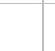
\includegraphics[max width=\textwidth]{2024_11_21_9c6d19831f6022e8f7beg-05(3)}
 &  & 
\includegraphics[max width=\textwidth]{2024_11_21_9c6d19831f6022e8f7beg-05(16)}
 &  & 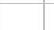
\includegraphics[max width=\textwidth]{2024_11_21_9c6d19831f6022e8f7beg-05(7)}
 & \(\square\) &  &  & 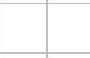
\includegraphics[max width=\textwidth]{2024_11_21_9c6d19831f6022e8f7beg-05(2)}
 \\
\hline
 &  &  &  &  &  &  &  &  &  &  &  &  &  &  &  &  &  &  &  &  &  &  &  &  &  &  & 
\includegraphics[max width=\textwidth]{2024_11_21_9c6d19831f6022e8f7beg-05(5)}
 & 
\includegraphics[max width=\textwidth]{2024_11_21_9c6d19831f6022e8f7beg-05(1)}
 &  &  & 
\includegraphics[max width=\textwidth]{2024_11_21_9c6d19831f6022e8f7beg-05(13)}
 \\
\hline
 &  &  &  &  &  &  &  &  &  &  &  &  & 
\includegraphics[max width=\textwidth]{2024_11_21_9c6d19831f6022e8f7beg-05(8)}
 &  &  &  &  &  &  &  &  &  & 
\includegraphics[max width=\textwidth]{2024_11_21_9c6d19831f6022e8f7beg-05(17)}
 &  &  &  & 
\includegraphics[max width=\textwidth]{2024_11_21_9c6d19831f6022e8f7beg-05(9)}
 & 
\includegraphics[max width=\textwidth]{2024_11_21_9c6d19831f6022e8f7beg-05(18)}
 &  &  & 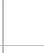
\includegraphics[max width=\textwidth]{2024_11_21_9c6d19831f6022e8f7beg-05}
 \\
\hline
 &  &  &  &  &  &  &  & 
\includegraphics[max width=\textwidth]{2024_11_21_9c6d19831f6022e8f7beg-05(15)}
 &  &  &  &  & 
\includegraphics[max width=\textwidth]{2024_11_21_9c6d19831f6022e8f7beg-05(6)}
 &  &  &  &  &  &  &  &  & 
\includegraphics[max width=\textwidth]{2024_11_21_9c6d19831f6022e8f7beg-05(4)}
 & 
\includegraphics[max width=\textwidth]{2024_11_21_9c6d19831f6022e8f7beg-05(11)}
 &  &  & 
\includegraphics[max width=\textwidth]{2024_11_21_9c6d19831f6022e8f7beg-05(14)}
 & 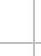
\includegraphics[max width=\textwidth]{2024_11_21_9c6d19831f6022e8f7beg-05(12)}
 & 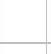
\includegraphics[max width=\textwidth]{2024_11_21_9c6d19831f6022e8f7beg-05(10)}
 &  &  &  \\
\hline
 &  &  &  &  &  &  &  &  &  &  &  &  &  &  &  &  &  &  &  &  &  &  &  &  &  &  &  &  &  &  &  \\
\hline
\end{tabular}
\end{center}

\(\qquad\)\\
\(\qquad\)\\
\(\qquad\)\\
\(\qquad\)\\
\(\qquad\)\\
\(\qquad\)\\
\(\qquad\)\\
\(\qquad\)\\
\(\qquad\)\\
\(\qquad\)\\
\(\qquad\)\\
\(\qquad\)\\
\(\qquad\)\\
\(\qquad\)

\begin{center}
\begin{tabular}{|c|l|c|c|c|}
\hline
\multirow{2}{*}{\begin{tabular}{c}
Wypetnia \\
egzaminator! \\
\end{tabular}} & Nr czynności & 4.1. & 4.2. & 4.3. \\
\cline { 2 - 5 }
 & Maks. liczba pkt & 1 & 1 & 1 \\
\cline { 2 - 5 }
 & Uzyskana liczba pkt &  &  &  \\
\hline
\end{tabular}
\end{center}

\section*{Zadanie 5. (7 pkt)}
Wierzchołki trójkąta równobocznego \(A B C\) są punktami paraboli \(y=-x^{2}+6 x\). Punkt \(C\) jest jej wierzchołkiem, a bok \(A B\) jest równoległy do osi Ox. Sporządź rysunek w układzie współrzędnych i wyznacz współrzędne wierzchołków tego trójkąta.\\

\includegraphics[max width=\textwidth, center]{2024_11_21_9c6d19831f6022e8f7beg-06}

\section*{Zadanie 6. (4 pkt)}
Niech \(A, B\) będą zdarzeniami o prawdopodobieństwach \(P(A)\) i \(P(B)\). Wykaż, że jeżeli \(P(A)=0,85\) i \(P(B)=0,75\), to prawdopodobieństwo warunkowe spełnia nierówność \(P(A \mid B) \geq 0,8\).\\

\includegraphics[max width=\textwidth, center]{2024_11_21_9c6d19831f6022e8f7beg-07}

\begin{center}
\begin{tabular}{|c|l|c|c|c|c|}
\hline
\multirow{2}{*}{\begin{tabular}{c}
Wypełnia \\
egzaminator! \\
\end{tabular}} & Nr czynności & 6.1. & 6.2. & 6.3. & 6.4. \\
\cline { 2 - 6 }
 & Maks. liczba pkt & 1 & 1 & 1 & 1 \\
\cline { 2 - 6 }
 & Uzyskana liczba pkt &  &  &  &  \\
\hline
\end{tabular}
\end{center}

\section*{Zadanie 7. (7 pkt)}
Dany jest układ równań: \(\left\{\begin{array}{l}m x-y=2 \\ x+m y=m\end{array}\right.\)\\
Dla każdej wartości parametru \(m\) wyznacz parę liczb \((x, y)\), która jest rozwiązaniem tego układu równań. Wyznacz najmniejszą wartość sumy \(x+y\) dla \(m \in\langle 2,4\rangle\).

\begin{center}
\begin{tabular}{|c|c|c|c|c|c|c|c|c|c|c|c|c|c|c|c|c|c|c|c|c|c|c|}
\hline
 &  &  &  &  &  &  &  &  &  &  &  &  &  &  &  &  &  &  &  &  &  &  \\
\hline
 &  &  &  &  &  &  &  &  &  &  &  &  &  &  &  &  &  &  &  &  &  &  \\
\hline
 &  &  &  &  &  &  &  &  &  &  &  &  &  &  &  &  &  &  &  &  &  &  \\
\hline
 &  &  &  &  &  &  &  &  &  &  &  &  &  &  &  &  &  &  &  &  &  &  \\
\hline
 &  &  &  &  &  &  &  &  &  &  &  &  &  &  &  &  &  &  &  &  &  &  \\
\hline
 &  &  &  &  &  &  &  &  &  &  &  &  &  &  &  &  &  &  &  &  &  &  \\
\hline
 &  &  &  &  &  &  &  &  &  &  &  &  &  &  &  &  &  &  &  &  &  &  \\
\hline
 &  &  &  &  &  &  &  &  &  &  &  &  &  &  &  &  &  &  &  &  &  &  \\
\hline
 &  &  &  &  &  &  &  &  &  &  &  &  &  &  &  &  &  &  &  &  &  &  \\
\hline
 &  &  &  &  &  &  &  &  &  &  &  &  &  &  &  &  &  &  &  &  &  &  \\
\hline
 &  &  &  &  &  &  &  &  &  &  &  &  &  &  &  &  &  &  &  &  &  &  \\
\hline
 &  &  &  &  &  &  &  &  &  &  &  &  &  &  &  &  &  &  &  &  &  &  \\
\hline
 &  &  &  &  &  &  &  &  &  &  &  &  &  &  &  &  &  &  &  &  &  &  \\
\hline
 &  &  &  &  &  &  &  &  &  &  &  &  &  &  &  &  &  &  &  &  &  &  \\
\hline
 &  &  &  &  &  &  &  &  &  &  &  &  &  &  &  &  &  &  &  &  &  &  \\
\hline
 &  &  &  &  &  &  &  &  &  &  &  &  &  &  &  &  &  &  &  &  &  &  \\
\hline
 &  &  &  &  &  &  &  &  &  &  &  &  &  &  &  &  &  &  &  &  &  &  \\
\hline
 &  &  &  &  &  &  &  &  &  &  &  &  &  &  &  &  &  &  &  &  &  &  \\
\hline
 &  &  &  &  &  &  &  &  &  &  &  &  &  &  &  &  &  &  &  &  &  &  \\
\hline
 &  &  &  &  &  &  &  &  &  &  &  &  &  &  &  &  &  &  &  &  &  &  \\
\hline
 &  &  &  &  &  &  &  &  &  &  &  &  &  &  &  &  &  &  &  &  &  &  \\
\hline
 &  &  &  &  &  &  &  &  &  &  &  &  &  &  &  &  &  &  &  &  &  &  \\
\hline
 &  &  &  &  &  &  &  &  &  &  &  &  &  &  &  &  &  &  &  &  &  &  \\
\hline
 &  &  &  &  &  &  &  &  &  &  &  &  &  &  &  &  &  &  &  &  &  &  \\
\hline
 &  &  &  &  &  &  &  &  &  &  &  &  &  &  &  &  &  &  &  &  &  &  \\
\hline
 &  &  &  &  &  &  &  &  &  &  &  &  &  &  &  &  &  &  &  &  &  &  \\
\hline
 &  &  &  &  &  &  &  &  &  &  &  &  &  &  &  &  &  &  &  &  &  &  \\
\hline
 &  &  &  &  &  &  &  &  &  &  &  &  &  &  &  &  &  &  &  &  &  &  \\
\hline
 &  &  &  &  &  &  &  &  &  &  &  &  &  &  &  &  &  &  &  &  &  &  \\
\hline
 &  &  &  &  &  &  &  &  &  &  &  &  &  &  &  &  &  &  &  &  &  &  \\
\hline
 &  &  &  &  &  &  &  &  &  &  &  &  &  &  &  &  &  &  &  &  &  &  \\
\hline
 &  &  &  &  &  &  &  &  &  &  &  &  &  &  &  &  &  &  &  &  &  &  \\
\hline
 &  &  &  &  &  &  &  &  &  &  &  &  &  &  &  &  &  &  &  &  &  &  \\
\hline
 &  &  &  &  &  &  &  &  &  &  &  &  &  &  &  &  &  &  &  &  &  &  \\
\hline
 &  &  &  &  &  &  &  &  &  &  &  &  &  &  &  &  &  &  &  &  &  &  \\
\hline
 &  &  &  &  &  &  &  &  &  &  &  &  &  &  &  &  &  &  &  &  &  &  \\
\hline
 &  &  &  &  &  &  &  &  &  &  &  &  &  &  &  &  &  &  &  &  &  &  \\
\hline
 &  &  &  &  &  &  &  &  &  &  &  &  &  &  &  &  &  &  &  &  &  &  \\
\hline
 &  &  &  &  &  &  &  &  &  &  &  &  &  &  &  &  &  &  &  &  &  &  \\
\hline
 &  &  &  &  &  &  &  &  &  &  &  &  &  &  &  &  &  &  &  &  &  &  \\
\hline
 &  &  &  &  &  &  &  &  &  &  &  &  &  &  &  &  &  &  &  &  &  &  \\
\hline
\end{tabular}
\end{center}

\begin{center}

\includegraphics[max width=\textwidth]{2024_11_21_9c6d19831f6022e8f7beg-09}
\end{center}

\begin{center}
\begin{tabular}{|c|l|c|c|c|c|c|c|c|}
\hline
\multirow{2}{*}{\begin{tabular}{c}
Wypelnia \\
egzaminator! \\
\end{tabular}} & Nr czynności & 7.1. & 7.2. & 7.3. & 7.4. & 7.5. & 7.6. & 7.7. \\
\cline { 2 - 9 }
 & Maks. liczba pkt & 1 & 1 & 1 & 1 & 1 & 1 & 1 \\
\cline { 2 - 9 }
 & Uzyskana liczba pkt &  &  &  &  &  &  &  \\
\hline
\end{tabular}
\end{center}

\section*{Zadanie 8. (3 pkt)}
Dana jest funkcja \(f\) określona wzorem \(f(x)=\frac{\sin ^{2} x-|\sin x|}{\sin x}\) dla \(x \in(0, \pi) \cup(\pi, 2 \pi)\).\\
a) Naszkicuj wykres funkcji \(f\).\\
b) Wyznacz miejsca zerowe funkcji \(f\).\\
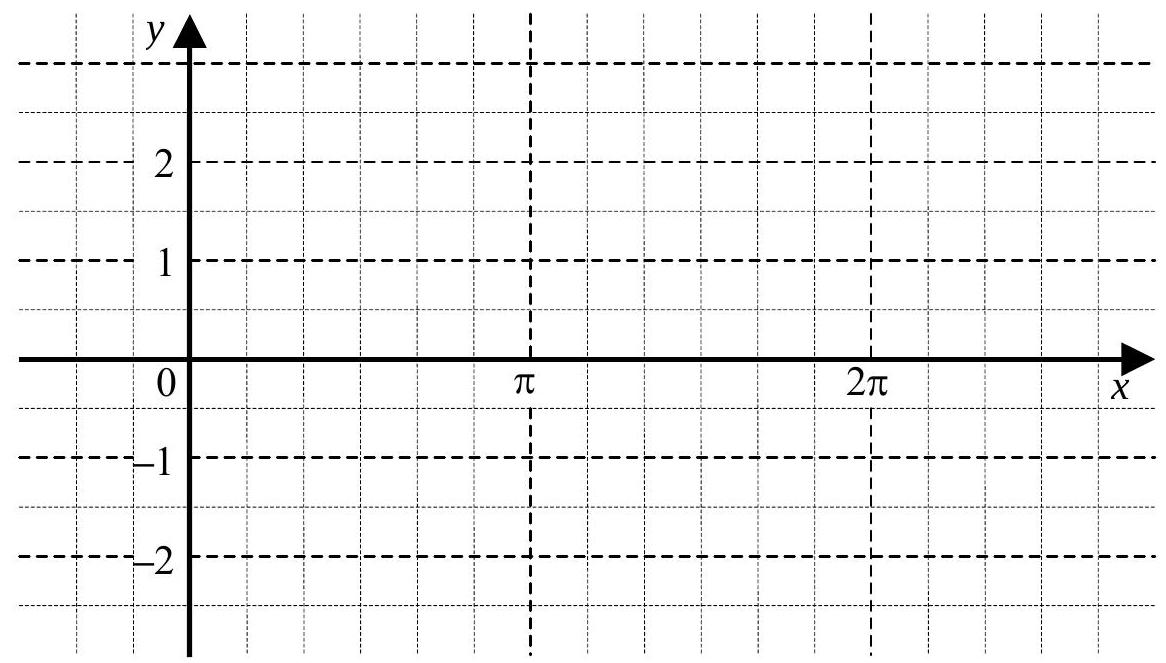
\includegraphics[max width=\textwidth, center]{2024_11_21_9c6d19831f6022e8f7beg-10}\\

\includegraphics[max width=\textwidth, center]{2024_11_21_9c6d19831f6022e8f7beg-10(1)}\\

\includegraphics[max width=\textwidth, center]{2024_11_21_9c6d19831f6022e8f7beg-11}

\begin{center}
\begin{tabular}{|c|l|c|c|c|}
\hline
\multirow{2}{*}{\begin{tabular}{c}
Wypelnia \\
egzaminator! \\
\end{tabular}} & Nr czynności & 8.1. & 8.2. & 8.3. \\
\cline { 2 - 5 }
 & Maks. liczba pkt & 1 & 1 & 1 \\
\cline { 2 - 5 }
 & Uzyskana liczba pkt &  &  &  \\
\hline
\end{tabular}
\end{center}

\section*{Zadanie 9. (3 pkt)}
Przedstaw wielomian \(W(x)=x^{4}-2 x^{3}-3 x^{2}+4 x-1\) w postaci iloczynu dwóch wielomianów stopnia drugiego o współczynnikach całkowitych i takich, że współczynniki przy drugich potęgach są równe jeden.\\

\includegraphics[max width=\textwidth, center]{2024_11_21_9c6d19831f6022e8f7beg-12}

\begin{center}
\begin{tabular}{|c|l|c|c|c|}
\hline
\multirow{2}{*}{\begin{tabular}{c}
Wypetnia \\
egzaminator! \\
\end{tabular}} & Nr czynności & 9.1. & 9.2. & 9.3. \\
\cline { 2 - 5 }
 & Maks. liczba pkt & 1 & 1 & 1 \\
\cline { 2 - 5 }
 & Uzyskana liczba pkt &  &  &  \\
\hline
\end{tabular}
\end{center}

\section*{Zadanie 10. (4 pkt)}
Na kole opisany jest romb. Stosunek pola koła do pola rombu wynosi \(\frac{\pi \sqrt{3}}{8}\). Wyznacz miarę kąta ostrego rombu.\\

\includegraphics[max width=\textwidth, center]{2024_11_21_9c6d19831f6022e8f7beg-13}

\begin{center}
\begin{tabular}{|c|l|c|c|c|c|}
\hline
\multirow{2}{*}{\begin{tabular}{c}
Wypełnia \\
egzaminator: \\
\end{tabular}} & Nr czynności & 10.1. & 10.2. & 10.3. & 10.4. \\
\cline { 2 - 6 }
 & Maks. liczba pkt & 1 & 1 & 1 & 1 \\
\cline { 2 - 6 }
 & Uzyskana liczba pkt &  &  &  &  \\
\hline
\end{tabular}
\end{center}

\section*{Zadanie 11. (4 pkt)}
Suma \(n\) początkowych wyrazów ciagu arytmetycznego \(\left(a_{n}\right)\) wyraża się wzorem \(S_{n}=2 n^{2}+n\) dla \(n \geq 1\).\\
a) Oblicz sumę 50 początkowych wyrazów tego ciagu o numerach parzystych: \(a_{2}+a_{4}+a_{6}+\ldots+a_{100}\).\\
b) Oblicz \(\lim _{n \rightarrow \infty} \frac{S_{n}}{3 n^{2}-2}\).\\

\includegraphics[max width=\textwidth, center]{2024_11_21_9c6d19831f6022e8f7beg-14}

\begin{center}
\begin{tabular}{|c|l|c|c|c|c|}
\hline
\multirow{2}{*}{\begin{tabular}{c}
Wypelnia \\
egzaminator! \\
\end{tabular}} & Nr czynności & 11.1. & 11.2. & 11.3. & 11.4. \\
\cline { 2 - 6 }
 & Maks. liczba pkt & 1 & 1 & 1 & 1 \\
\cline { 2 - 6 }
 & Uzyskana liczba pkt &  &  &  &  \\
\hline
\end{tabular}
\end{center}

\section*{BRUDNOPIS}

\end{document}